\documentclass{standalone}

\usepackage[euler-digits]{eulervm}

\usepackage{tikz}
\tikzset{every node/.style={circle,draw,minimum size=6mm,inner sep=0pt}}
\tikzset{t/.style={rectangle}}
\tikzset{l/.style={above,draw=none,font=\small}}
\tikzset{a/.style={red,very thick,->,>=latex}}
\begin{document}
    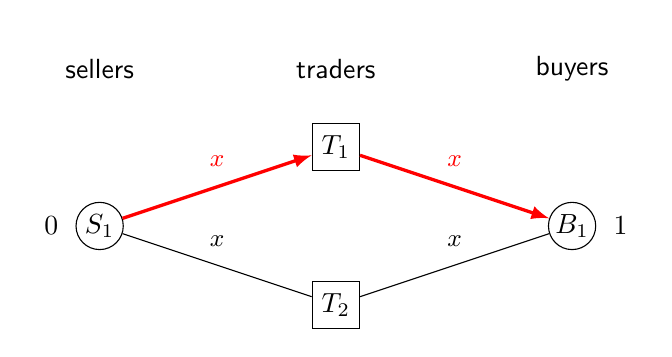
\begin{tikzpicture}[font=\sffamily]
        \node[draw=none] (S) at (-3,4) {sellers};
        \node[draw=none] (B) at (3,4) {buyers};
        \node[draw=none] (T) at (0,4) {traders};
      \node[label=left:{$0$}] (S2) at (-3,2) {$S_1$}; 
      \node[label=right:{$1$}] (B2) at (3,2) {$B_1$}; 
      \node[t] (T1) at (0,3) {$T_1$}; 
      \node[t] (T2) at (0,1) {$T_2$}; 
      \draw[a] (S2) -- node[l] {$x$} (T1);
      \draw (S2) -- node[l] {$x$} (T2);
      \draw[a] (T1) -- node[l] {$x$} (B2);
      \draw (T2) -- node[l] {$x$} (B2);
    \end{tikzpicture}
\end{document}
